\documentclass{standalone}
\usepackage{tikz}
\usepackage{ctex,siunitx}
\usepackage{tkz-euclide}
\usepackage{amsmath}
\usetikzlibrary{patterns, calc}
\usetikzlibrary {decorations.pathmorphing, decorations.pathreplacing, decorations.shapes,}
\begin{document}
\small
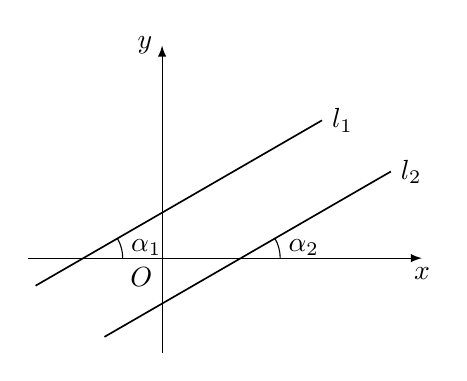
\begin{tikzpicture}[>=latex,scale=1.0]
  \draw[thin,->](-1.7,0)--(3.3,0)node[below]{$x$};
  \draw[thin,->](0,-1.2)--(0,2.7)node[left]{$y$};
  \node at (0,0)[below left]{$O$};
  \draw[semithick](-1,0)--++(30:3.5)node[right]{$l_1$};
  \draw[semithick](-1,0)--++(-150:0.7);
  \draw[semithick](1,0)--++(30:2.2)node[right]{$l_2$};
  \draw[semithick](1,0)--++(-150:2.0);
  \draw(-0.5,0)arc(0:30:0.5)node[midway,right]{$\alpha_1$};
  \draw(1.5,0)arc(0:30:0.5)node[midway,right]{$\alpha_2$};
\end{tikzpicture}
\end{document}